We can define a ray as having two components:
$$\Vec{O} \text{ a three dimensional vector representing the ray's origin}$$
$$\text{and}$$
$$\hat{D} \text{ a \textbf{normalized} three dimensional vector representing the ray's direction}$$
These two components can be combined to provide a unified definition:
$$ \Vec{O} + t\hat{D} $$
where $t$ is a scalar which represents a distance along the ray's direction from the origin. \\ \\
\noindent
To render a scene, we must cast at a ray for each pixel on the screen in order to determine the pixel's color. The ray's origin will be defined as the camera's position while the ray's direction must be calculated by mapping pixel coordinates on to the camera's viewport. First we can define our screen dimensions with $S_w$ being the screen's width in pixels and $S_h$ being the screen's height in pixels. Considering that the orientation of the camera's viewport will be determined by the camera's direction, we can find the relative horizontal and vertical unit vectors of the viewport ($\hat{H}$ and $\hat{U}$ respectively) using vector cross products as follows:

$$\hat{H} = \begin{bmatrix} 0 \\ 1 \\ 0 \end{bmatrix} \times \hat{V}  $$
$$\hat{U} = \hat{H} \times \hat{V}$$

\noindent
For example, if the camera direction $\hat{V}$ is $\begin{bmatrix} 0 \\ 0 \\ 1 \end{bmatrix}$, then $\hat{H}$ will be $\begin{bmatrix} 1 \\ 0 \\ 0 \end{bmatrix}$ and $\hat{U}$ will be $\begin{bmatrix} 0 \\ 1 \\ 0 \end{bmatrix}$

\noindent
Based on these vectors, we can begin calculating the direction and origin of our camera ray's. First, we know that $\Vec{O} = \Vec{P}$ because all camera rays will originate from the camera's position. Next, we can calculate the bottom left corner of our viewport in world space as
$$\Vec{B} = -\frac{w}{2}\hat{H} - \frac{h}{2}\hat{U}$$
Given a screen pixel coordinate ($x$, $y$), we are now ready to determine the corresponding camera ray's direction.
$$\Vec{A} = \Vec{B} + (w \frac{x}{S_w})\hat{H} + (h \frac{y}{S_h})\hat{U} + z\hat{V}$$
Normalizing $\Vec{A}$ gives us our final direction:
$$\hat{D} = \frac{\Vec{A}}{|\Vec{A}|} = \frac{\Vec{B} + (w \frac{x}{S_w})\hat{H} + (h \frac{y}{S_h})\hat{U} + z\hat{V}}{|\Vec{B} + (w \frac{x}{S_w})\hat{H} + (h \frac{y}{S_h})\hat{U} + z\hat{V}|}$$
Now, we can define our camera ray for a particular pixel ($x$, $y$) as:
$$R = \Vec{P} + t(\frac{\Vec{B} + (w \frac{x}{S_w})\hat{H} + (h \frac{y}{S_h})\hat{U} + z\hat{V}}{|\Vec{B} + (w \frac{x}{S_w})\hat{H} + (h \frac{y}{S_h})\hat{U} + z\hat{V}|})$$

\begin{figure}[H]
    \centering
    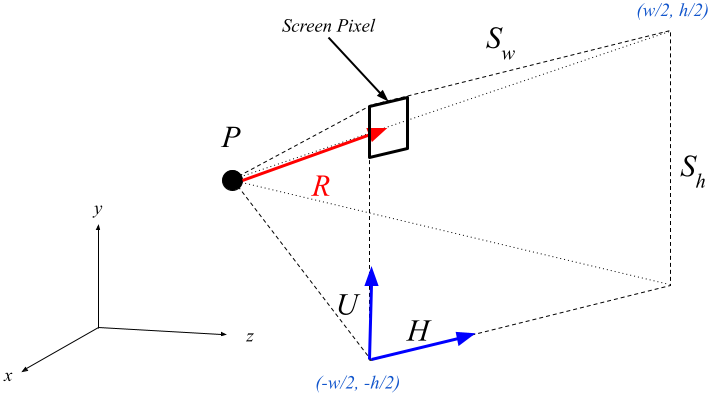
\includegraphics[scale=0.5]{figures/CameraRays.png}
    \caption{Diagram of ray generation and mapping from screen to viewport space. Pixel's near the center of the screen will have fairly straight corresponding camera rays while pixels near the corners will have angled camera rays, simulating distortion in the camera's peripheral vision.}
    \label{fig:cam_rays}
\end{figure}
\noindent
To begin generating an image, we must calculate the corresponding ray for each pixel and trace its path in the scene over time as demonstrated in the illustration below.

\begin{figure}[H]
    \centering
    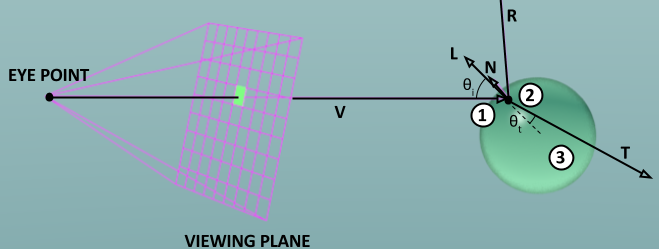
\includegraphics[scale=0.5]{figures/ApproachIllustration.png}
    \caption{Process of determining pixel color based on the interactions of camera ray $v$ with the scene (Wikimedia Commons)}
    \label{fig:approach}
\end{figure}
\noindent
For now, given that we have yet to define any scene objects, we will assign a color, represented by a three dimensional vector in the form $\begin{bmatrix}\text{red}, \text{green}, \text{blue} \end{bmatrix}$ where each component ranges from 0 to 1, to each pixel based on the $y$ component of the pixel's corresponding camera ray direction. When placing the camera at the point $\begin{bmatrix}0, 0, -1 \end{bmatrix}$ with direction $\begin{bmatrix}0,  0, 1 \end{bmatrix}$, $z = 1$, and $h = 2, w = 2\frac{16}{9}$ (the standard 16:9 aspect ratio), this produces the following image when giving higher $y$ components a darker blue color and lower $y$ components a lighter blue color in order to simulate the appearance of a clear sky.

\begin{figure}[H]
    \centering
    
\includegraphics[scale=0.4]{figures/FirstImage.png}
    \caption{First image generated by varying each pixel's color based on the $y$ component of the pixel's corresponding camera ray's direction.}
    \label{fig:first_image}
\end{figure}